\documentclass[aspectratio=169]{beamer}

\usetheme{default}
\usecolortheme{dove}

\setbeamertemplate{navigation symbols}{}
\setbeamertemplate{footline}{%
  \hfill\insertframenumber\,/\,\inserttotalframenumber\hspace{0.5em}\vspace{0.5em}%
}

\definecolor{popblue}{RGB}{52, 101, 164}
\definecolor{sampred}{RGB}{204, 0, 0}
\definecolor{paramgreen}{RGB}{0, 140, 70}
\definecolor{warnred}{RGB}{180, 40, 40}
\definecolor{orange1}{RGB}{220, 120, 0}
\definecolor{violet1}{RGB}{120, 50, 160}

\setbeamercolor{frametitle}{fg=popblue}
\setbeamercolor{title}{fg=popblue}

\usepackage{pgfplots}
\usepackage{tikz}
\usetikzlibrary{shapes, arrows.meta, positioning, calc, decorations.pathreplacing, patterns}
\pgfplotsset{compat=1.18}
\usepackage{amsmath, amssymb}

\title{Lecture 2b: MAP Estimation}
\subtitle{Priors, Posteriors, and the Regularization Connection}
\date{}

\begin{document}

% ============================================================
\begin{frame}
\titlepage
\end{frame}

% ============================================================
\begin{frame}
\frametitle{Where We Are}
\begin{center}
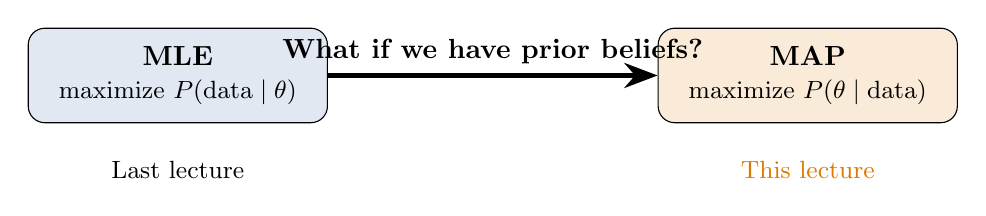
\begin{tikzpicture}[
  box/.style={draw, rounded corners=6pt, minimum width=3.8cm, minimum height=1.2cm, align=center, font=\normalsize}
]
  \node[box, fill=popblue!15] (mle) at (-4, 0) {\textbf{MLE}\\{\small maximize $P(\text{data} \mid \theta)$}};
  \node[box, fill=orange1!15] (map) at (4, 0) {\textbf{MAP}\\{\small maximize $P(\theta \mid \text{data})$}};

  \draw[-{Stealth}, very thick, line width=2pt] (mle) -- (map)
    node[midway, above, font=\normalsize\bfseries] {What if we have prior beliefs?};

  \node[font=\small] at (-4, -1.2) {Last lecture};
  \node[font=\small, orange1] at (4, -1.2) {This lecture};
\end{tikzpicture}
\end{center}
\end{frame}

% ============================================================
\section{Bayes' Theorem for Parameters}

\begin{frame}
\frametitle{Bayes' Theorem for Parameters}
\begin{center}
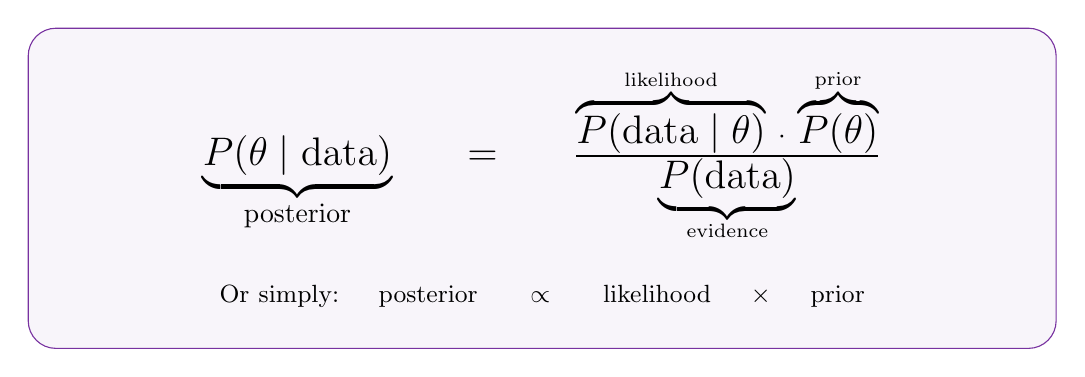
\begin{tikzpicture}
  \node[draw=violet1, fill=violet1!5, rounded corners=10pt, text width=12cm, align=center, inner sep=15pt] {
    {\Large
    $\underbrace{P(\theta \mid \text{data})}_{\text{posterior}} \;=\; \frac{\overbrace{P(\text{data} \mid \theta)}^{\text{likelihood}} \;\cdot\; \overbrace{P(\theta)}^{\text{prior}}}{\underbrace{P(\text{data})}_{\text{evidence}}}$
    }\\[15pt]
    \small Or simply: \quad $\text{posterior} \;\propto\; \text{likelihood} \;\times\; \text{prior}$
  };
\end{tikzpicture}
\end{center}
\end{frame}

\begin{frame}
\frametitle{The Three Ingredients}
\begin{center}
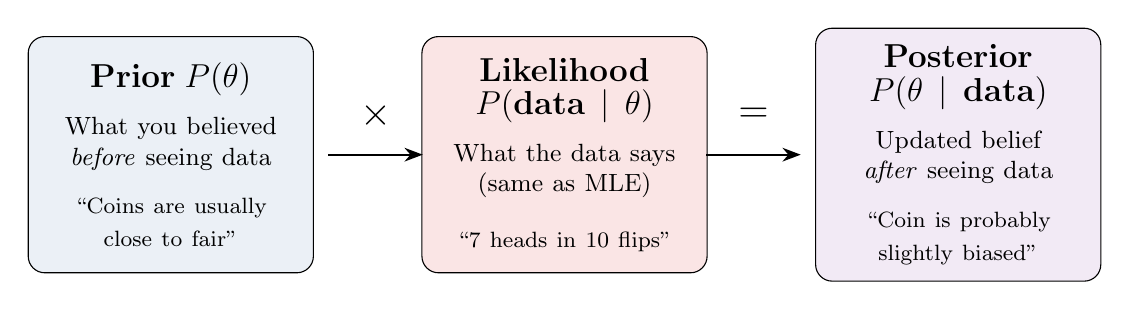
\begin{tikzpicture}[
  ibox/.style={draw, rounded corners=6pt, minimum width=3.5cm, minimum height=3cm, align=center, text width=3.2cm, inner sep=6pt}
]
  \node[ibox, fill=popblue!10] at (-5, 0) {
    \textbf{\large Prior $P(\theta)$}\\[6pt]
    \small What you believed\\
    \textit{before} seeing data\\[8pt]
    \footnotesize ``Coins are usually\\
    close to fair''
  };
  \node[ibox, fill=sampred!10] at (0, 0) {
    \textbf{\large Likelihood}\\
    \textbf{\large $P(\text{data} \mid \theta)$}\\[6pt]
    \small What the data says\\
    (same as MLE)\\[8pt]
    \footnotesize ``7 heads in 10 flips''
  };
  \node[ibox, fill=violet1!10] at (5, 0) {
    \textbf{\large Posterior}\\
    \textbf{\large $P(\theta \mid \text{data})$}\\[6pt]
    \small Updated belief\\
    \textit{after} seeing data\\[8pt]
    \footnotesize ``Coin is probably\\
    slightly biased''
  };

  \draw[-{Stealth}, thick] (-3, 0) -- (-1.8, 0);
  \node[font=\Large] at (-2.4, 0.5) {$\times$};
  \draw[-{Stealth}, thick] (1.8, 0) -- (3, 0);
  \node[font=\Large] at (2.4, 0.5) {$=$};
\end{tikzpicture}
\end{center}
\end{frame}

\begin{frame}
\frametitle{Visualizing the Update: Coin Bias}
\begin{center}
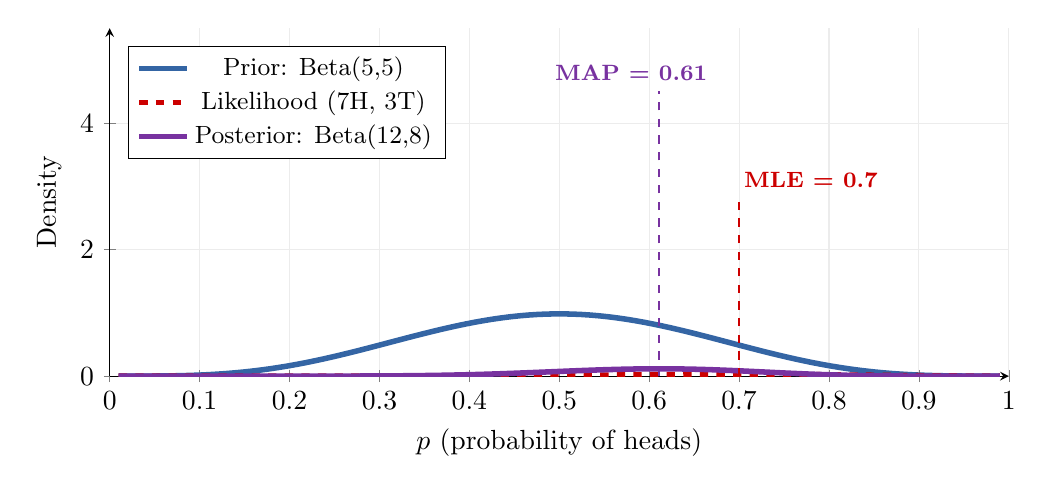
\begin{tikzpicture}
  \begin{axis}[
    width=13cm, height=6cm,
    xlabel={$p$ (probability of heads)},
    ylabel={Density},
    xmin=0, xmax=1,
    ymin=0, ymax=5.5,
    axis lines=left,
    legend style={at={(0.02,0.95)}, anchor=north west, font=\small},
    grid=major, grid style={gray!15},
    every axis plot/.append style={line width=2pt, samples=100}
  ]
    % Prior: Beta(5,5) - centered at 0.5
    \addplot[popblue, domain=0.01:0.99] {(x^4 * (1-x)^4) / 0.00397};
    \addlegendentry{Prior: Beta(5,5)}

    % Likelihood: 7 heads in 10 (proportional)
    \addplot[sampred, dashed, domain=0.01:0.99] {3.2 * x^7 * (1-x)^3 / 0.267};
    \addlegendentry{Likelihood (7H, 3T)}

    % Posterior: Beta(12,8)
    \addplot[violet1, domain=0.01:0.99] {(x^11 * (1-x)^7) / 0.0000516};
    \addlegendentry{Posterior: Beta(12,8)}

    % MAP and MLE markers
    \draw[thick, violet1, dashed] (axis cs:0.611, 0) -- (axis cs:0.611, 4.5);
    \node[font=\footnotesize\bfseries, violet1] at (axis cs:0.58, 4.8) {MAP = 0.61};

    \draw[thick, sampred, dashed] (axis cs:0.7, 0) -- (axis cs:0.7, 2.8);
    \node[font=\footnotesize\bfseries, sampred] at (axis cs:0.78, 3.1) {MLE = 0.7};
  \end{axis}
\end{tikzpicture}
\end{center}
\small Prior pulls the estimate from 0.7 toward 0.5. The posterior is a \textbf{compromise}.
\end{frame}

% ============================================================
\section{MAP Estimation}

\begin{frame}
\frametitle{MAP = Mode of the Posterior}
\begin{center}
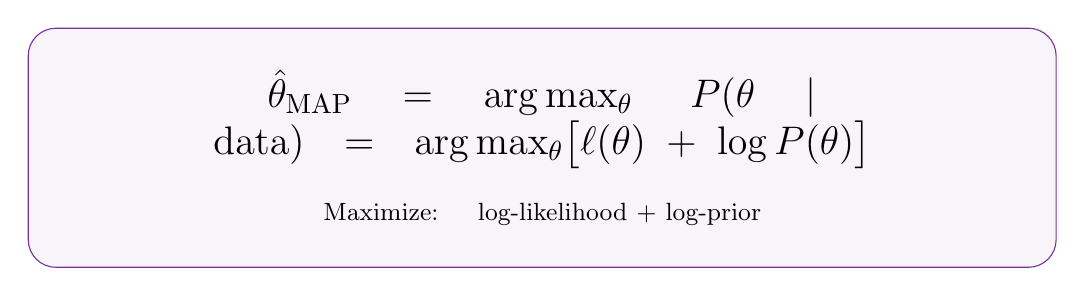
\begin{tikzpicture}
  \node[draw=violet1, fill=violet1!5, rounded corners=10pt, text width=12cm, align=center, inner sep=15pt] {
    {\Large
    $\hat{\theta}_{\text{MAP}} = \arg\max_\theta \; P(\theta \mid \text{data}) = \arg\max_\theta \bigl[\ell(\theta) + \log P(\theta)\bigr]$
    }\\[12pt]
    \small Maximize: \quad log-likelihood $+$ log-prior
  };
\end{tikzpicture}
\end{center}

\vspace{0.5cm}
\begin{center}
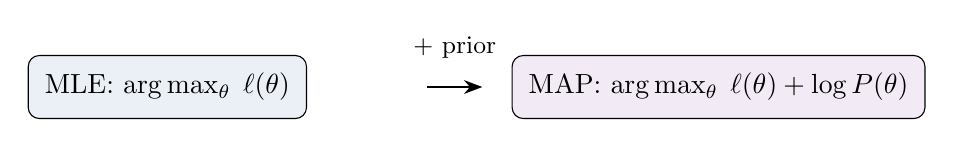
\begin{tikzpicture}[
  cbox/.style={draw, rounded corners=4pt, minimum height=0.8cm, align=center, font=\normalsize, inner sep=6pt}
]
  \node[cbox, fill=popblue!10] at (-3, 0) {MLE: $\arg\max_\theta \; \ell(\theta)$};
  \node[cbox, fill=violet1!10] at (4, 0) {MAP: $\arg\max_\theta \; \ell(\theta) + \log P(\theta)$};
  \draw[-{Stealth}, thick] (0.3, 0) -- (1, 0);
  \node[font=\small] at (0.65, 0.5) {$+$ prior};
\end{tikzpicture}
\end{center}

\vspace{0.3cm}
\small MAP = MLE with an extra penalty/bonus term from the prior.
\end{frame}

\begin{frame}
\frametitle{When Does the Prior Matter?}
\begin{center}
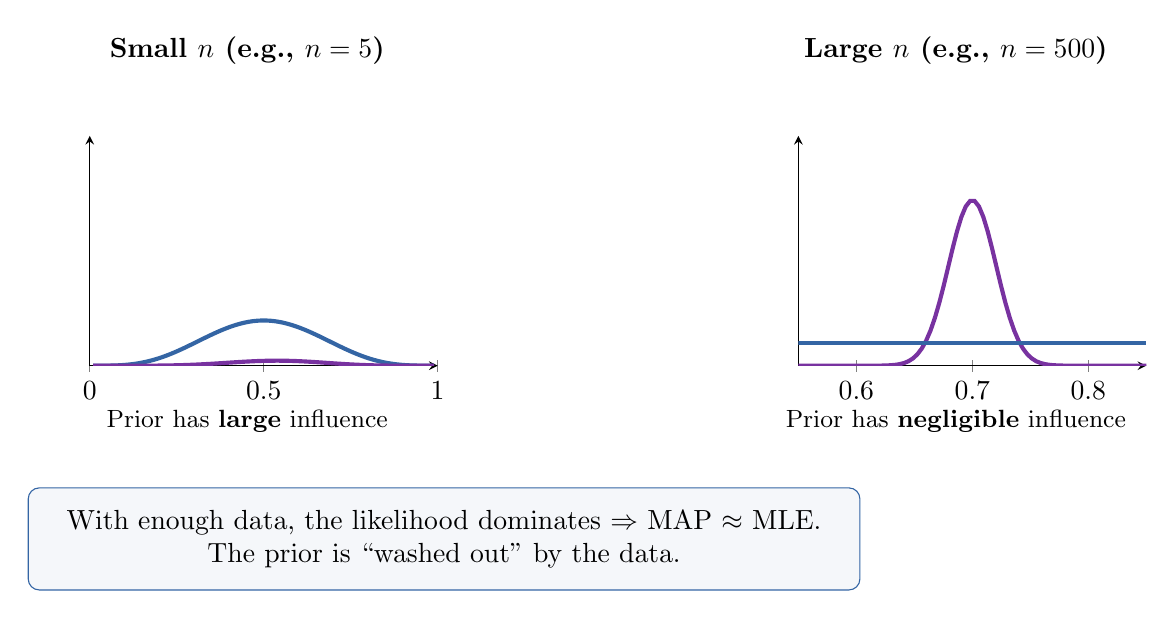
\begin{tikzpicture}
  % Small n
  \begin{scope}[xshift=-4.5cm]
    \node[font=\bfseries] at (2, 4) {Small $n$ (e.g., $n=5$)};
    \begin{axis}[
      width=6cm, height=4.5cm,
      xmin=0, xmax=1, ymin=0, ymax=5,
      axis lines=left,
      xtick={0,0.5,1}, ytick=\empty,
      every axis plot/.append style={line width=1.5pt, samples=80},
      at={(0,0)}
    ]
      \addplot[popblue, domain=0.01:0.99] {(x^4*(1-x)^4)/0.00397};
      \addplot[violet1, domain=0.01:0.99] {(x^7*(1-x)^6)/0.00116};
    \end{axis}
    \node[font=\small] at (2, -0.7) {Prior has \textbf{large} influence};
  \end{scope}

  % Large n
  \begin{scope}[xshift=4.5cm]
    \node[font=\bfseries] at (2, 4) {Large $n$ (e.g., $n=500$)};
    \begin{axis}[
      width=6cm, height=4.5cm,
      xmin=0.55, xmax=0.85, ymin=0, ymax=25,
      axis lines=left,
      xtick={0.6, 0.7, 0.8}, ytick=\empty,
      every axis plot/.append style={line width=1.5pt, samples=80},
      at={(0,0)}
    ]
      % Posterior with n=500: very narrow, centered near MLE
      \addplot[violet1, domain=0.55:0.85] {exp(-500*(x-0.7)^2 / (2*0.7*0.3)) * 18};
      % Prior: almost flat in this range
      \addplot[popblue, domain=0.55:0.85] {2.5};
    \end{axis}
    \node[font=\small] at (2, -0.7) {Prior has \textbf{negligible} influence};
  \end{scope}

  % Bottom message
  \node[draw=popblue, fill=popblue!5, rounded corners=4pt, text width=10cm, align=center, font=\normalsize, inner sep=8pt] at (0, -2.2) {
    With enough data, the likelihood dominates $\Rightarrow$ MAP $\approx$ MLE.\\
    The prior is ``washed out'' by the data.
  };
\end{tikzpicture}
\end{center}
\end{frame}

% ============================================================
\section{Regularization as MAP}

\begin{frame}
\frametitle{The Key Connection: Regularization = MAP}
\begin{center}
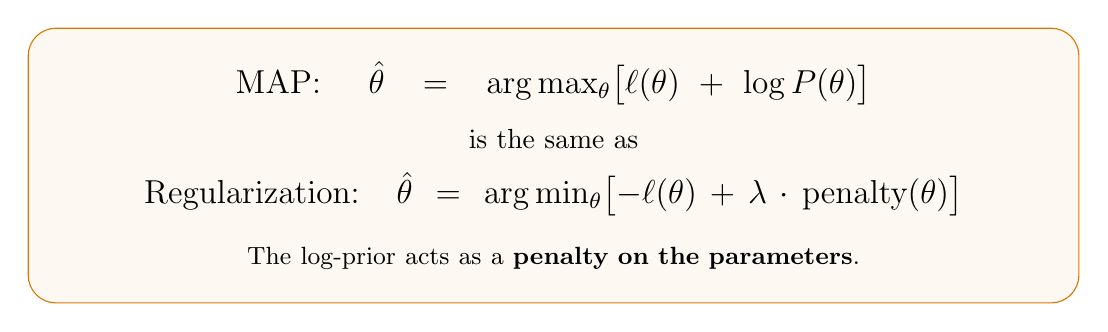
\begin{tikzpicture}
  \node[draw=orange1, fill=orange1!5, rounded corners=10pt, text width=12.5cm, align=center, inner sep=12pt] {
    {\large MAP: $\;\hat{\theta} = \arg\max_\theta \bigl[\ell(\theta) + \log P(\theta)\bigr]$}\\[8pt]
    is the same as\\[8pt]
    {\large Regularization: $\;\hat{\theta} = \arg\min_\theta \bigl[-\ell(\theta) + \lambda \cdot \text{penalty}(\theta)\bigr]$}\\[10pt]
    \small The log-prior acts as a \textbf{penalty on the parameters}.
  };
\end{tikzpicture}
\end{center}
\end{frame}

\begin{frame}
\frametitle{Gaussian Prior $\Leftrightarrow$ Ridge (L2) Regression}
\begin{center}
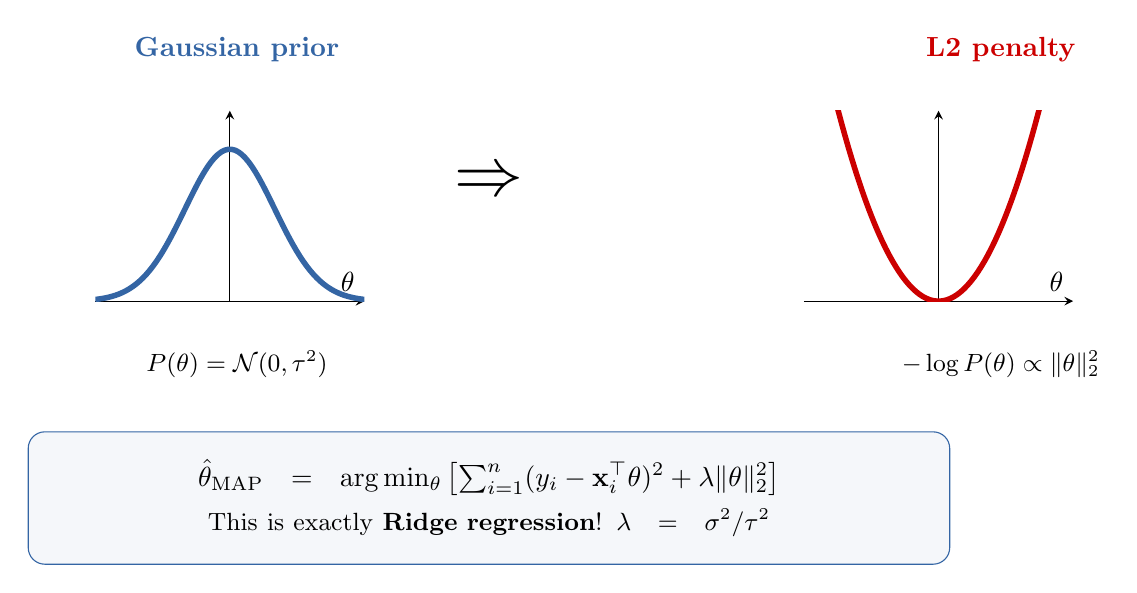
\begin{tikzpicture}
  % Left: prior
  \begin{scope}[xshift=-5cm]
    \node[font=\bfseries, popblue] at (1.8, 3.2) {Gaussian prior};
    \begin{axis}[
      width=5cm, height=4cm,
      xmin=-3, xmax=3, ymin=0, ymax=0.5,
      axis lines=middle,
      xtick=\empty, ytick=\empty,
      every axis plot/.append style={line width=2pt, samples=80},
      at={(0,0)},
      xlabel={$\theta$}
    ]
      \addplot[popblue, domain=-3:3] {exp(-x^2/2)/sqrt(2*pi)};
    \end{axis}
    \node[font=\small] at (1.8, -0.8) {$P(\theta) = \mathcal{N}(0, \tau^2)$};
  \end{scope}

  % Arrow
  \node[font=\Huge] at (0, 1.5) {$\Rightarrow$};

  % Right: penalty
  \begin{scope}[xshift=4cm]
    \node[font=\bfseries, sampred] at (2.5, 3.2) {L2 penalty};
    \begin{axis}[
      width=5cm, height=4cm,
      xmin=-3, xmax=3, ymin=0, ymax=5,
      axis lines=middle,
      xtick=\empty, ytick=\empty,
      every axis plot/.append style={line width=2pt, samples=80},
      at={(0,0)},
      xlabel={$\theta$}
    ]
      \addplot[sampred, domain=-3:3] {x^2};
    \end{axis}
    \node[font=\small] at (2.5, -0.8) {$-\log P(\theta) \propto \|\theta\|_2^2$};
  \end{scope}

  % Bottom equation
  \node[draw=popblue, fill=popblue!5, rounded corners=6pt, text width=11cm, align=center, inner sep=10pt] at (0, -2.5) {
    $\hat{\theta}_{\text{MAP}} = \arg\min_\theta \left[\sum_{i=1}^n(y_i - \mathbf{x}_i^\top\theta)^2 + \lambda\|\theta\|_2^2\right]$\\[4pt]
    \small This is exactly \textbf{Ridge regression}! $\lambda = \sigma^2/\tau^2$
  };
\end{tikzpicture}
\end{center}
\end{frame}

\begin{frame}
\frametitle{Laplace Prior $\Leftrightarrow$ Lasso (L1) Regression}
\begin{center}
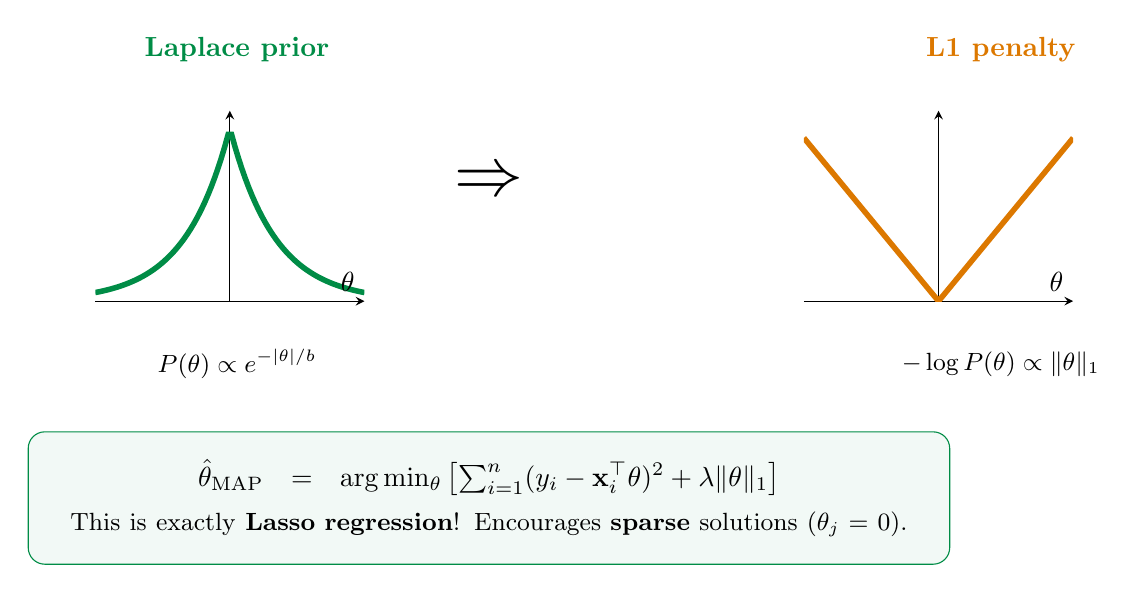
\begin{tikzpicture}
  % Left: prior
  \begin{scope}[xshift=-5cm]
    \node[font=\bfseries, paramgreen] at (1.8, 3.2) {Laplace prior};
    \begin{axis}[
      width=5cm, height=4cm,
      xmin=-3, xmax=3, ymin=0, ymax=0.55,
      axis lines=middle,
      xtick=\empty, ytick=\empty,
      every axis plot/.append style={line width=2pt, samples=80},
      at={(0,0)},
      xlabel={$\theta$}
    ]
      \addplot[paramgreen, domain=-3:3] {0.5*exp(-abs(x))};
    \end{axis}
    \node[font=\small] at (1.8, -0.8) {$P(\theta) \propto e^{-|\theta|/b}$};
  \end{scope}

  % Arrow
  \node[font=\Huge] at (0, 1.5) {$\Rightarrow$};

  % Right: penalty
  \begin{scope}[xshift=4cm]
    \node[font=\bfseries, orange1] at (2.5, 3.2) {L1 penalty};
    \begin{axis}[
      width=5cm, height=4cm,
      xmin=-3, xmax=3, ymin=0, ymax=3.5,
      axis lines=middle,
      xtick=\empty, ytick=\empty,
      every axis plot/.append style={line width=2pt, samples=80},
      at={(0,0)},
      xlabel={$\theta$}
    ]
      \addplot[orange1, domain=-3:3] {abs(x)};
    \end{axis}
    \node[font=\small] at (2.5, -0.8) {$-\log P(\theta) \propto \|\theta\|_1$};
  \end{scope}

  % Bottom equation
  \node[draw=paramgreen, fill=paramgreen!5, rounded corners=6pt, text width=11cm, align=center, inner sep=10pt] at (0, -2.5) {
    $\hat{\theta}_{\text{MAP}} = \arg\min_\theta \left[\sum_{i=1}^n(y_i - \mathbf{x}_i^\top\theta)^2 + \lambda\|\theta\|_1\right]$\\[4pt]
    \small This is exactly \textbf{Lasso regression}! Encourages \textbf{sparse} solutions ($\theta_j = 0$).
  };
\end{tikzpicture}
\end{center}
\end{frame}

\begin{frame}
\frametitle{The Regularization Map}
\begin{center}
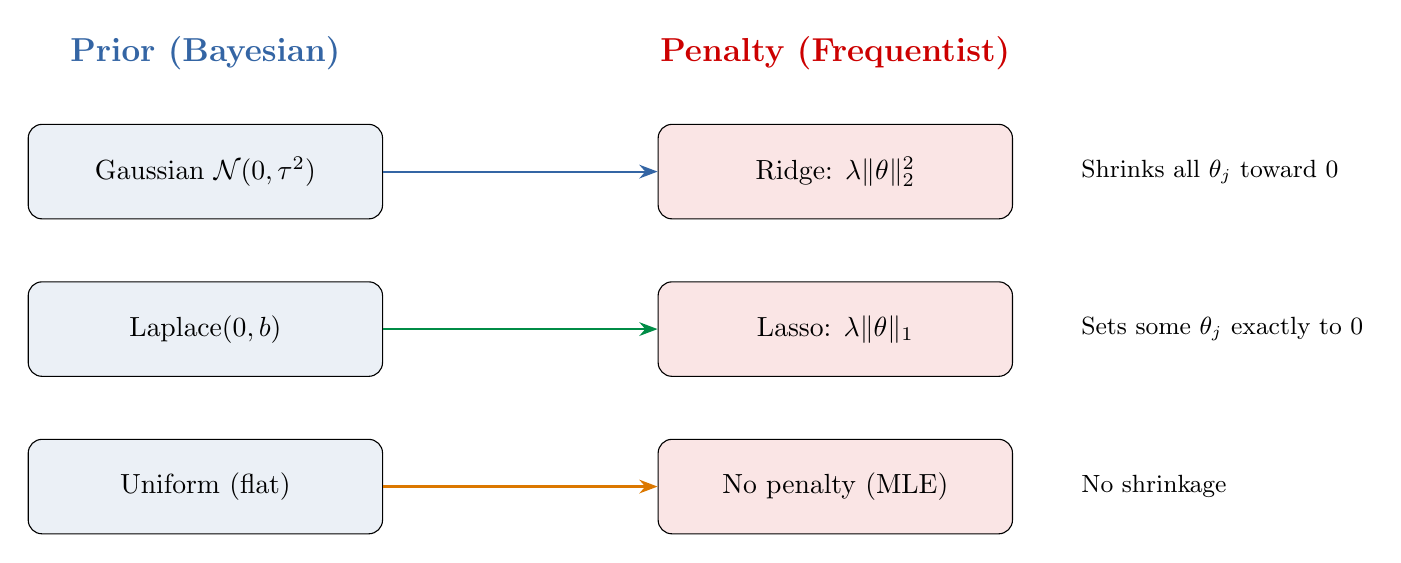
\begin{tikzpicture}[
  mbox/.style={draw, rounded corners=5pt, minimum width=4.5cm, minimum height=1.2cm, align=center, font=\normalsize, inner sep=6pt}
]
  % Prior column
  \node[font=\large\bfseries, popblue] at (-4, 3.5) {Prior (Bayesian)};
  \node[mbox, fill=popblue!10] (g) at (-4, 2) {Gaussian $\mathcal{N}(0, \tau^2)$};
  \node[mbox, fill=popblue!10] (l) at (-4, 0) {Laplace$(0, b)$};
  \node[mbox, fill=popblue!10] (u) at (-4, -2) {Uniform (flat)};

  % Regularizer column
  \node[font=\large\bfseries, sampred] at (4, 3.5) {Penalty (Frequentist)};
  \node[mbox, fill=sampred!10] (r) at (4, 2) {Ridge: $\lambda\|\theta\|_2^2$};
  \node[mbox, fill=sampred!10] (la) at (4, 0) {Lasso: $\lambda\|\theta\|_1$};
  \node[mbox, fill=sampred!10] (no) at (4, -2) {No penalty (MLE)};

  \draw[-{Stealth}, thick, popblue] (g) -- (r);
  \draw[-{Stealth}, thick, paramgreen] (l) -- (la);
  \draw[-{Stealth}, thick, orange1] (u) -- (no);

  % Effect column
  \node[font=\small, right] at (7, 2) {Shrinks all $\theta_j$ toward 0};
  \node[font=\small, right] at (7, 0) {Sets some $\theta_j$ exactly to 0};
  \node[font=\small, right] at (7, -2) {No shrinkage};
\end{tikzpicture}
\end{center}
\end{frame}

\begin{frame}
\frametitle{Visualizing Ridge Shrinkage}
\begin{center}
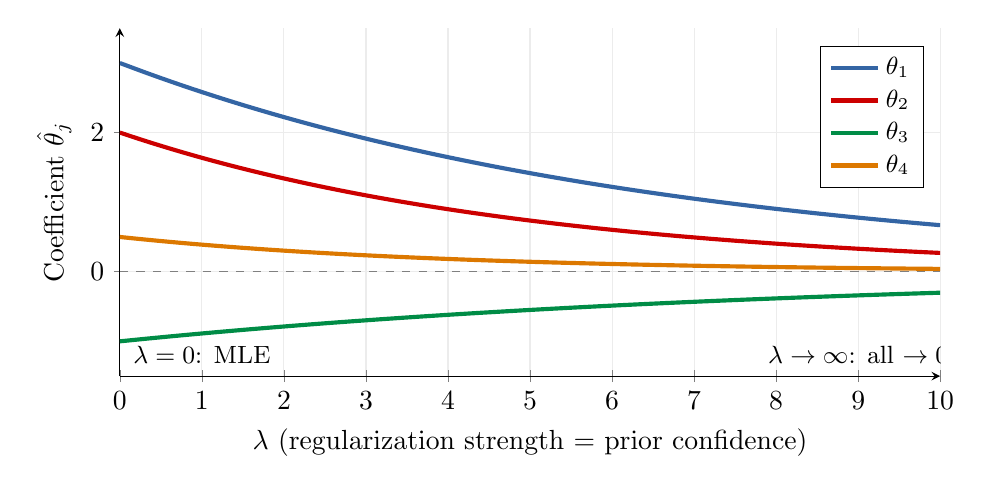
\begin{tikzpicture}
  \begin{axis}[
    width=12cm, height=6cm,
    xlabel={$\lambda$ (regularization strength = prior confidence)},
    ylabel={Coefficient $\hat{\theta}_j$},
    xmin=0, xmax=10,
    ymin=-1.5, ymax=3.5,
    axis lines=left,
    grid=major, grid style={gray!15},
    every axis plot/.append style={line width=1.5pt, samples=80},
    legend style={at={(0.98,0.95)}, anchor=north east, font=\small}
  ]
    % Several coefficients shrinking toward 0
    \addplot[popblue, domain=0:10] {3 * exp(-0.15*x)};
    \addlegendentry{$\theta_1$}
    \addplot[sampred, domain=0:10] {2 * exp(-0.2*x)};
    \addlegendentry{$\theta_2$}
    \addplot[paramgreen, domain=0:10] {-1 * exp(-0.12*x)};
    \addlegendentry{$\theta_3$}
    \addplot[orange1, domain=0:10] {0.5 * exp(-0.25*x)};
    \addlegendentry{$\theta_4$}

    % Zero line
    \draw[dashed, gray] (axis cs:0,0) -- (axis cs:10,0);

    % Labels
    \node[font=\small] at (axis cs:1, -1.2) {$\lambda = 0$: MLE};
    \node[font=\small] at (axis cs:9, -1.2) {$\lambda \to \infty$: all $\to 0$};
  \end{axis}
\end{tikzpicture}
\end{center}
\small Increasing $\lambda$ = stronger prior = more shrinkage = less overfitting (but more bias).
\end{frame}

% ============================================================
\section{MLE vs MAP vs Full Bayesian}

\begin{frame}
\frametitle{Three Philosophies}
\begin{center}
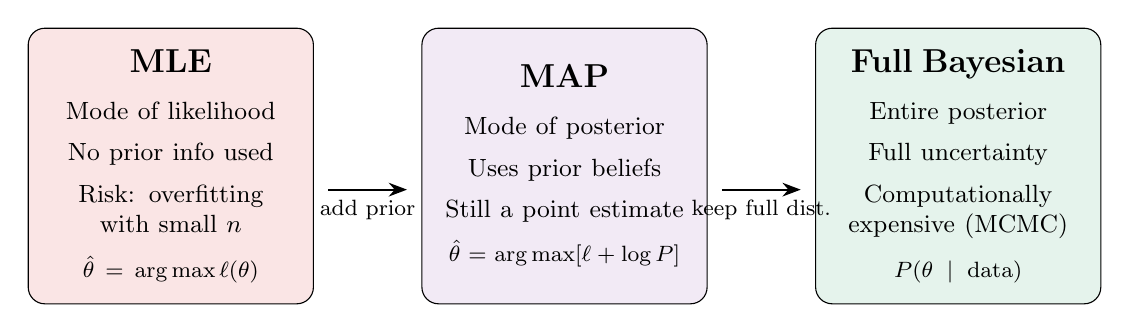
\begin{tikzpicture}[
  pbox/.style={draw, rounded corners=6pt, minimum width=3.5cm, minimum height=3.5cm, align=center, text width=3.2cm, inner sep=6pt}
]
  \node[pbox, fill=sampred!10] at (-5, 0) {
    \textbf{\large MLE}\\[6pt]
    \small Mode of likelihood\\[4pt]
    No prior info used\\[4pt]
    Risk: overfitting\\with small $n$\\[4pt]
    \footnotesize $\hat{\theta} = \arg\max \ell(\theta)$
  };
  \node[pbox, fill=violet1!10] at (0, 0) {
    \textbf{\large MAP}\\[6pt]
    \small Mode of posterior\\[4pt]
    Uses prior beliefs\\[4pt]
    Still a point estimate\\[4pt]
    \footnotesize $\hat{\theta} = \arg\max [\ell + \log P]$
  };
  \node[pbox, fill=paramgreen!10] at (5, 0) {
    \textbf{\large Full Bayesian}\\[6pt]
    \small Entire posterior\\[4pt]
    Full uncertainty\\[4pt]
    Computationally\\expensive (MCMC)\\[4pt]
    \footnotesize $P(\theta \mid \text{data})$
  };

  \draw[-{Stealth}, thick] (-3, -0.3) -- (-2, -0.3) node[midway, below, font=\footnotesize] {add prior};
  \draw[-{Stealth}, thick] (2, -0.3) -- (3, -0.3) node[midway, below, font=\footnotesize] {keep full dist.};
\end{tikzpicture}
\end{center}
\end{frame}

\begin{frame}
\frametitle{When to Use What}
\begin{center}
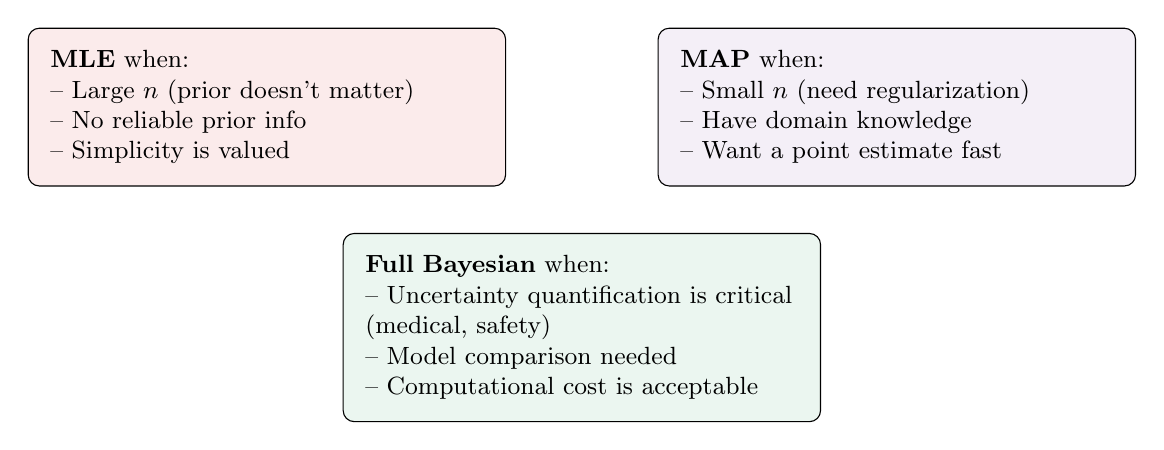
\begin{tikzpicture}[
  when/.style={draw, rounded corners=4pt, minimum height=1.5cm, text width=5.5cm, align=left, inner sep=8pt, font=\small}
]
  \node[when, fill=sampred!8] at (-4, 2) {
    \textbf{MLE} when:\\
    -- Large $n$ (prior doesn't matter)\\
    -- No reliable prior info\\
    -- Simplicity is valued
  };
  \node[when, fill=violet1!8] at (4, 2) {
    \textbf{MAP} when:\\
    -- Small $n$ (need regularization)\\
    -- Have domain knowledge\\
    -- Want a point estimate fast
  };
  \node[when, fill=paramgreen!8] at (0, -0.8) {
    \textbf{Full Bayesian} when:\\
    -- Uncertainty quantification is critical (medical, safety)\\
    -- Model comparison needed\\
    -- Computational cost is acceptable
  };
\end{tikzpicture}
\end{center}
\end{frame}

% ============================================================
\section{Practical}

\begin{frame}
\frametitle{Practical: Priors and Posteriors}
\begin{center}
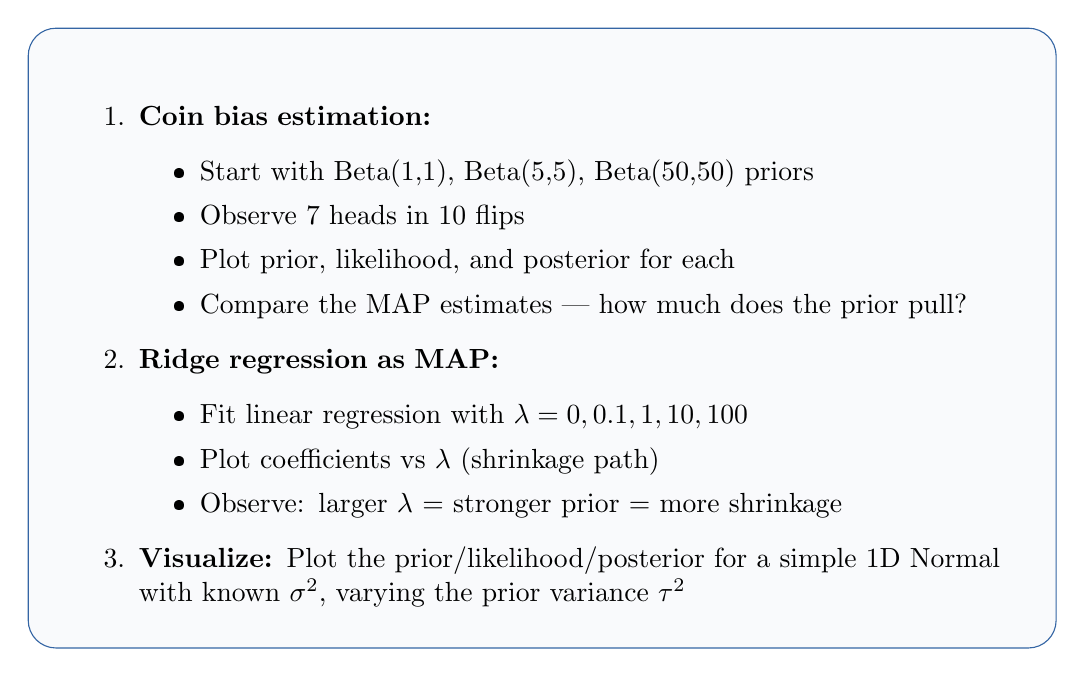
\begin{tikzpicture}
  \node[draw=popblue, fill=popblue!3, rounded corners=10pt, text width=12cm, align=left, inner sep=15pt] {
    \begin{enumerate}
      \item \textbf{Coin bias estimation:}
        \begin{itemize}
          \item Start with Beta(1,1), Beta(5,5), Beta(50,50) priors
          \item Observe 7 heads in 10 flips
          \item Plot prior, likelihood, and posterior for each
          \item Compare the MAP estimates --- how much does the prior pull?
        \end{itemize}
      \item \textbf{Ridge regression as MAP:}
        \begin{itemize}
          \item Fit linear regression with $\lambda = 0, 0.1, 1, 10, 100$
          \item Plot coefficients vs $\lambda$ (shrinkage path)
          \item Observe: larger $\lambda$ = stronger prior = more shrinkage
        \end{itemize}
      \item \textbf{Visualize:} Plot the prior/likelihood/posterior for a simple 1D Normal with known $\sigma^2$, varying the prior variance $\tau^2$
    \end{enumerate}
  };
\end{tikzpicture}
\end{center}
\end{frame}

\begin{frame}
\begin{center}
  {\Huge\bfseries\textcolor{popblue}{Questions?}}

  \vspace{1cm}

  {\large Next lecture: Estimator Quality --- Bias, Variance, and the Tradeoff}
\end{center}
\end{frame}

\end{document}
